\documentclass{article}
%\usepackage{enumitem}
\usepackage[table]{xcolor}
\usepackage{listings,multicol}
\usepackage{amsfonts}
\usepackage{latexsym}
\usepackage{fullpage}
\usepackage{graphicx}
%\usepackage{paralist}
\usepackage{tikz-timing}
\usepackage{tabto}
\usepackage[utf8]{inputenc}
\usepackage[T1]{fontenc}
\usepackage{filecontents}
\usepackage[backend=biber,style=ieee]{biblatex}
\usepackage{caption}
\usepackage{subcaption}
\usepackage[brazilian]{babel}
\lstset{language=C}

\graphicspath{{images/}}

% Default margins are too wide all the way around. I reset them here
\setlength{\topmargin}{-.5in}
\setlength{\textheight}{9in}
\setlength{\oddsidemargin}{.125in}
\setlength{\textwidth}{6.25in}

\lstset{literate=
  {á}{{\'a}}1 {é}{{\'e}}1 {í}{{\'i}}1 {ó}{{\'o}}1 {ú}{{\'u}}1
  {Á}{{\'A}}1 {É}{{\'E}}1 {Í}{{\'I}}1 {Ó}{{\'O}}1 {Ú}{{\'U}}1
  {à}{{\`a}}1 {è}{{\`e}}1 {ì}{{\`i}}1 {ò}{{\`o}}1 {ù}{{\`u}}1
  {À}{{\`A}}1 {È}{{\'E}}1 {Ì}{{\`I}}1 {Ò}{{\`O}}1 {Ù}{{\`U}}1
  {ä}{{\"a}}1 {ë}{{\"e}}1 {ï}{{\"i}}1 {ö}{{\"o}}1 {ü}{{\"u}}1
  {Ä}{{\"A}}1 {Ë}{{\"E}}1 {Ï}{{\"I}}1 {Ö}{{\"O}}1 {Ü}{{\"U}}1
  {â}{{\^a}}1 {ê}{{\^e}}1 {î}{{\^i}}1 {ô}{{\^o}}1 {û}{{\^u}}1
  {Â}{{\^A}}1 {Ê}{{\^E}}1 {Î}{{\^I}}1 {Ô}{{\^O}}1 {Û}{{\^U}}1
  {œ}{{\oe}}1 {Œ}{{\OE}}1 {æ}{{\ae}}1 {Æ}{{\AE}}1 {ß}{{\ss}}1
  {ű}{{\H{u}}}1 {Ű}{{\H{U}}}1 {ő}{{\H{o}}}1 {Ő}{{\H{O}}}1
  {ç}{{\c c}}1 {Ç}{{\c C}}1 {ø}{{\o}}1 {å}{{\r a}}1 {Å}{{\r A}}1
  {€}{{\euro}}1 {£}{{\pounds}}1 {«}{{\guillemotleft}}1
  {»}{{\guillemotright}}1 {ñ}{{\~n}}1 {Ñ}{{\~N}}1 {¿}{{?`}}1
  {ã}{{\~a}}1 {Ã}{{\~A}}1
}

\definecolor{backgroundColour}{rgb}{0.95,0.95,0.92}

\lstdefinestyle{CStyle}{
    backgroundcolor=\color{backgroundColour},   
    basicstyle=\footnotesize,
    breakatwhitespace=false,         
    breaklines=true,                 
    captionpos=b,                    
    keepspaces=true,                 
    numbers=left,                    
    numbersep=5pt,                  
    showspaces=false,                
    showstringspaces=false,
    showtabs=false,                  
    tabsize=2,
    language=C
}

\renewcommand{\lstlistingname}{Exemplo}

% Defining references here

\begin{filecontents}{\jobname.bib}
@article{singh2014,
author = {Dhananjay, Singh and Gaurav, Tripathi},
year = {2014},
month = {03},
pages = {},
title = {A Survey of Internet-of-Things: Future Vision, Architecture, Challenges and Services},
journaltitle = {2014 IEEE World Forum on Internet of Things, WF-IoT 2014}
}
@online{arduinoblog,
author = {Arduino},
title = {Arduino Blog},
year = {2017},
url = {https://blog.arduino.cc},
OPTnote = {Acessado em 24 de Abril de 2017}
}
@article{santanna2012,
author = {Francisco Sant’Anna and
Noemi de La Rocque Rodriguez and
Roberto Ierusalimschy},
title = {CÉU: Embedded, Safe, and
Reactive},
journaltitle = {Monografias em Ciência da Computação},
year = {2012},
volume = {9},
issn = {0103-9741}
}
@online{githubceuarduino,
author = {Francisco Sant'Anna},
title = {GitHub Céu-Arduino},
year = {2017},
url = {https://github.com/fsantanna/ceu-arduino},
note = {Acessado em 24 de Abril de 2017}
}
@article{wortmann2015,
author = {Felix Wortmann and Kristina Flütcher},
year = {2015},
pages = {221-224},
title = {Internet of Things - Technology and Value Added},
journaltitle = {Business \& Information Systems Engineering},
volume = {57},
issue = {3}
}
@periodical{chui2010,
editor = {Michael Chui and Markus Löffer and Roger Roberts},
title = {The Internet of Things},
year = {2010},
series = {McKinsey Quarterly},
month = {Março},
url = {https://www.mckinsey.com/industries/high-tech/our-insights/the-internet-of-things}
}
@ARTICLE{edwards1997, 
author={S. Edwards and L. Lavagno and E. A. Lee and A. Sangiovanni-Vincentelli}, 
journal={Proceedings of the IEEE}, 
title={Design of embedded systems: formal models, validation, and synthesis}, 
year={1997}, 
volume={85}, 
number={3}, 
pages={366-390}, 
keywords={application specific integrated circuits;computer architecture;formal specification;formal verification;logic design;real-time systems;systems analysis;ASIC;application-specific integrated circuits;concurrent design process;embedded software;embedded systems design;formal models;formal validation;heterogeneous systems;reactive real-time system design;specification;Application software;Application specific integrated circuits;Computer architecture;Consumer electronics;Embedded computing;Embedded system;Hardware;Microcontrollers;Real time systems;Safety}, 
doi={10.1109/5.558710}, 
ISSN={0018-9219}, 
month={Mar},}
@online{githubceu,
author = {Francisco Sant'Anna},
title = {GitHub Céu},
year = {2017},
url = {https://github.com/fsantanna/ceu},
note = {Acessado em 24 de Abril de 2017}
}
@manual{atmegadatasheet,
author = {AtMel},
title = {AtMel ATmega328/P DATASHEET},
year = {2016},
organization = {ATMel},
}

\end{filecontents}

\addbibresource{\jobname.bib}

% End defining references

\begin{document}

\begin{titlepage}

\newcommand{\HRule}{\rule{\linewidth}{0.5mm}} % Defines a new command for the horizontal lines, change thickness here

\center % Center everything on the page
 
%----------------------------------------------------------------------------------------
%	HEADING SECTIONS
%----------------------------------------------------------------------------------------

\textsc{\LARGE Pontifícia Universidade Católica do Rio de Janeiro}\\[1.5cm] % Name of your university/college
\textsc{\Large Projeto Final de Graduação de Engenharia da Computação}\\[0.5cm] % Minor heading such as course title

\textsc{\large Departamento de Informática - DI \\ Centro Técnico Científico - CTC \\ Curso de Engenharia da Computação}\\[0.5cm] % Major heading such as course name


%----------------------------------------------------------------------------------------
%	TITLE SECTION
%----------------------------------------------------------------------------------------

\HRule \\[0.4cm]
{ \huge \bfseries Aplicação em Sistemas Distribuídos
utilizando biblioteca e driver próprios,
baseados em interrupções desenvolvido
em Céu para o microcontrolador Arduino}\\[0.4cm] % Title of your document
\HRule \\[1.5cm]
 
%----------------------------------------------------------------------------------------
%	AUTHOR SECTION
%----------------------------------------------------------------------------------------

\begin{minipage}{0.4\textwidth}
\begin{flushleft} \large
\emph{Aluno:}\\
Guilherme \textsc{Simas} % Your name
\end{flushleft}
\end{minipage}
~
\begin{minipage}{0.4\textwidth}
\begin{flushright} \large
\emph{Orientador:} \\
Ana \textsc{Lúcia de Moura} % Supervisor's Name
\end{flushright}
\end{minipage}\\[4cm]

% If you don't want a supervisor, uncomment the two lines below and remove the section above
%\Large \emph{Author:}\\
%John \textsc{Smith}\\[3cm] % Your name

%----------------------------------------------------------------------------------------
%	DATE SECTION
%----------------------------------------------------------------------------------------

{\large \today}\\[3cm] % Date, change the \today to a set date if you want to be precise

%----------------------------------------------------------------------------------------
%	LOGO SECTION
%----------------------------------------------------------------------------------------

%\includegraphics{Logo}\\[1cm] % Include a department/university logo - this will require the graphicx package
 
%----------------------------------------------------------------------------------------

\vfill % Fill the rest of the page with whitespace

\end{titlepage}

\newpage % Dedicatória

\begin{flushright}

\vspace*{\fill}

\textit{\LARGE Agradecimentos estarão descritos nesse bloco de texto. Caso o bloco de texto seja grande demais espera-se que ele pule linhas e continue se guiando pela margem direita}

\vspace*{\fill}

\end{flushright}

\newpage

\tableofcontents{}

\newpage

\section{Introdução}	


\tab Existem várias definições do termo “Internet das
Coisas”, porém a grande maioria delas compartilha a ideia de que a conexão e troca de dados
entre elementos é parte vital do conceito. Por esse motivo, a área de Sistemas Distribuídos possui um
papel importantíssimo nesse desenvolvimento, já que toda aplicação deve ser capaz de trocar
mensagens e informação segura e corretamente de forma a se sincronizar, e de forma escalável. \cite{singh2014}
Outro ponto sobre a escalabilidade de aplicações em Internet das Coisas é a necessidade de unidades
computacionais de custo baixo e consumo eficiente de energia. Por esse motivo microcontroladores
são outra parte vital do desenvolvimento de soluções, apresentando, entre outras vantagens, uma
facilidade na programação devido a bibliotecas e drivers já implementados e disponibilizados.
Microcontroladores são capazes de processamento de dados por possuírem processadores e de
serem facilmente integrados com sensores e atuadores, possuindo hardware especializado para
interfacear com esses componentes.
\par Muitas ferramentas de desenvolvimento fornecidos para microcontroladores incluem rotinas que causam um bloqueio na
aplicação, ou seja, enquanto está realizando a chamada correspondente àquela funcionalidade, o
software entra em um estado onde realiza tarefas inúteis até que o hardware conclua sua
parte. Esse comportamento é indesejável visto que a aplicação desperdiça tempo aguardando o
hardware enquanto poderia estar realizando outras tarefas como, por exemplo, um processamento de
dados recebidos por uma mensagem, ou a troca de mensagens em si. Essa ineficiência marca um
desperdício de tempo e consumo de energia. O motivo pelo qual tal comportamento bloqueante é utilizado é pela simplicidade decorrente da programação sequencial.
\par O bloqueio de aplicações é um desafio enfrentado frequentemente em aplicações que envolvem
sistemas nos quais o tempo de processamento ou reação a estímulos externos é pertinente ao
funcionamento da aplicação. O paradigma de programação orientada a eventos é utilizado como abordagem nessas situações. Em uma aplicação orientada a eventos, o sistema segue
seu fluxo normal até a chegada de um “evento”, como a chegada de uma mensagem, ou a conclusão
de um trabalho por parte do hardware. A chegada de tal evento emite uma interrupção no sistema, que
irá executar uma rotina de tratamento desse evento, e após terminado, irá retomar seu fluxo normal
de execução, a partir de onde estava no momento da interrupção. Esse paradigma busca evitar que
quaisquer estímulos sejam ignorados involuntariamente pela aplicação ou que ciclos computacionais
sejam desperdiçados. Essa estruturação introduz uma espécie de paralelismo e imprevisibilidade no
fluxo de execução da aplicação, algo que linguagens comumente utilizadas para programação de
sistemas embarcados, como C, não fazem um bom papel de representar, por serem historicamente
procedurais (espera-se que o fluxo de execução siga naturalmente a ordem de leitura do código, a
linha de baixo imediatamente seguindo a execução da linha de cima).
\par Dentre um número enorme de microcontroladores, a plataforma Arduino possui uma comunidade estabelecida de desenvolvedores e é open-source. Contribuições na forma de
exemplos de aplicações e desenvolvimento de drivers e bibliotecas são frequentes e são o que tornam
a comunidade tão bem-sucedida. Por último, a plataforma é de fácil acesso e muitas vezes utilizada
como parâmetro, devido à sua popularidade. \cite{arduinoblog}
\par Céu é uma linguagem de programação estruturada síncrona reativa, onde a orientação a eventos é
inerente à programação, assim como o paralelismo entre seções de código que surgem com esse
paradigma, como mencionado anteriormente. A linguagem, portanto, faz um ótimo papel de
implementar a orientação a eventos. Outro benefício de Céu é o fato de que a ordem de execução de
trechos de programa que estão descritos para rodar em paralelo é previsível dado a chegada de um
determinado evento. \cite{santanna2012} Devido às vantagens dessas características para a programação de
componentes de sistemas embarcados, se encontra desenvolvido um kit de desenvolvimento em Céu para
uma família de microcontroladores, Arduino, chamada Céu-Arduino.
\par Céu-Arduino permite a programação de microcontroladores Arduino utilizando a linguagem Céu, o
que facilita a programação orientada a eventos. Céu-Arduino, porém, não reimplementa os drivers e
bibliotecas já desenvolvidos para Arduino, e, portanto, não pode impedir o
bloqueio da aplicação que é consequência da chamada de funções bloqueantes pré-desenvolvidas. A
re-implementação desses módulos eliminaria mais uma possibilidade de bloqueio de uma aplicação
que as utilize. \cite{githubceuarduino}
\par Esse trabalho propõe reimplementar drivers e bibliotecas de Arduino, que atualmente causam
bloqueio da aplicação, de forma a que esse bloqueio não ocorra mais. A abordagem utilizada nesse
desenvolvimento foi do uso de interrupções suportadas por hardware especializado com orientação a
eventos e, por esse motivo, a linguagem escolhida para esse desenvolvimento foi Céu-Arduino. Os
resultados desse desenvolvimento foram publicados na página open-source de desenvolvimento do
kit, para que futuros desenvolvedores possam fazer uso de tais módulos em suas próprias aplicações
e objetivos.
\par Por fim, desenvolvemos uma aplicação em Sistemas Distribuídos para exemplificar a pertinência
dos módulos desenvolvidos. A aplicação consiste em uma rede de sensores e atuadores na
plataforma Arduino, utilizando troca de mensagens. A aplicação escolhida como estudo de caso foi um sistema de iluminação inteligente. Esse trabalho tem como meta servir como uma contribuição
para a comunidade desenvolvedora de sistemas embarcados e de aplicações de IoT, assim como
desenvolvedores da plataforma Arduino. \cite{wortmann2015} \cite{chui2010} \cite{edwards1997} \cite{githubceu} \cite{atmegadatasheet}

\section{Fundamentos}

\subsection{Bloqueio de Aplicações}

\tab Bloqueios em chamadas de drivers de microcontroladores são comumente causados por implementações que usam polling para checar se a operação foi concluída. Polling é caracterizado
quando o software constantemente checa um estado, aguardando uma mudança, para só então
prosseguir. Funcionalidades de hardware especializado em microcontroladores costumam sinalizar sua
conclusão mudando o estado de um registrador, caracterizando uma flag. Implementações não-bloqueantes de chamadas de drivers podem envolver fazer com que a mudança de estado da flag cause
uma interrupção, de modo que o software não precisa ficar no estado de polling e possa usar o tempo
para realizar outras operações na aplicação, só retornando à chamada do driver quando este concluiu
sua tarefa. Caso não haja nenhuma tarefa a ser realizada, o microcontrolador pode entrar em um
modo de baixo consumo de energia, portanto sempre há ganhos por utilizar a abordagem não-
bloqueante.

\begin{figure}[t]
\centering
\begin{subfigure}[b]{.5\textwidth}
  \centering
  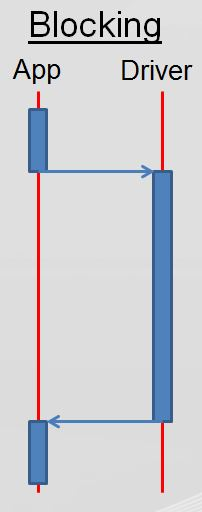
\includegraphics[width=.4\linewidth]{BlockingSequence}
  \caption{Comportamento bloqueante}
  \label{fig:sub1}
\end{subfigure}%
\begin{subfigure}[b]{.5\textwidth}
  \centering
  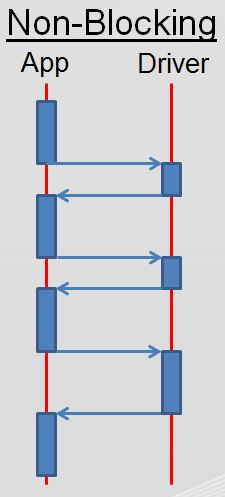
\includegraphics[width=.4\linewidth]{NonBlockingSequence}
  \caption{Comportamento não-bloqueante}
  \label{fig:sub2}
\end{subfigure}
\caption{Comparação entre comportamento bloqueante e não-bloqueante}
\label{fig:test}
\end{figure}

\par Existem microcontroladores, como Arduino, que oferecem suporte a interrupções externas. A implementação desse suporte se dá em um pino do microcontrolador que dispara uma interrupção na presença de uma mudança de estado específica no pino. Para que um driver de um dispositivo forneça suporte a interrupções, portanto, basta que o dispositivo possua uma saída que emita uma mudança de estado na ocorrência de eventos relevantes. Ao conectar esta saída ao pino de interrupção externa do microcontrolador, é possível mapear um evento do dispositivo a uma interrupção do microcontrolador, permitindo a orientação a evento que torna possível evitar o bloqueio desnecessário da aplicação.
\par Esse modelo é uma convenção de ambas as partes e se repete nos microcontroladores mais populares do mercado, incluindo Arduino, assim como nos dispositivos externos fabricados para sistemas embarcados. Isso facilita o desenvolvimento de drivers e bibliotecas para ambas as partes.
\par Kits de desenvolvimento para microcontroladores que ajudam a abstrair a implementação do hardware do programador são sempre benéficos por tornarem o processo de desenvolvimento de aplicações para aquele módulo mais simples e acessível. Contudo, os drivers e bibliotecas disponibilizados pela própria Arduino apresentam atualmente funções e módulos que causam o bloqueio da aplicação por utilizarem a técnica de polling, embora existam reimplementações por parte da comunidade de alguns desses módulos de forma a eliminar o bloqueio.

\subsection{Arduino}

\tab Arduino é uma plataforma eletrônica open-source que foca em hardware e software de fácil aprendizado e acesso. Comumente utilizado para prototipação, Arduino conta atualmente com a contribuição de uma vasta comunidade que realiza os mais diversos projetos de sistemas-embarcados, de complexidade variada. \cite{arduinoblog}
\par A plataforma consiste em uma placa de prototipação com um microcontrolador embarcado. A placa possui pinos de entrada e saída com grande foco em GPIO (General Purpose Input and Output). A programação se dá via linguagem C adaptada com bilbiotecas e drivers, com a implementação obrigatória de duas funções que definem a aplicação (ver Exemplo \ref{estruturaarduino}). O conjunto de ferramentas permite a abstração de elementos específicos à programação de microcontroladores como acessos a registradores, por exemplo, permitindo um desenvolvimento mais alto-nível, acessível e portável. Arduino oferece dezenas de placas diferentes, de especificações variadas de forma a atender diversas demandas. A placa mais popular, porém, é a Arduino Uno, que possuiu embarcado o microcontrolador ATmega328P, da Atmel \cite{atmegadatasheet}. Todo o desenvolvimento realizado neste projeto foi focado únicamente na portabilidade para o ambiente deste microcontrolador, embora a adaptação para outros produtos da Arduino seja facilitada pela proposta de portabilidade da empresa.
\begin{lstlisting}[style=CStyle,label=estruturaarduino,caption=Estrutura de uma aplicação Arduino]
void setup(void){
  // Esse bloco é executado uma vez somente, na inicialização da aplicação
}
void loop(void){
  // Este bloco é repetido em loop durante toda o período de execução da aplicação
}
\end{lstlisting}
\par Como já mencionado, microcontroladores Arduino são programados em um ambiente de linguagem C, uma linguagem procedural. A linguagem segue a lógica de procedência temporal e lógica dos comandos por ordem de leitura, o que significa que espera-se que um comando só seja executado quando o precedente acima dele termina sua execução. Esse método sequencial de programação reforça a proposta de simplicidade da plataforma Arduino. 
\par Como estudo de caso tenhamos uma aplicação cujo objetivo é piscar um LED até o momento que o usuário aperte um botão. O Exemplo \ref{orientacaoevento1} apresenta uma implementação simples utilizando as funções disponíveis da plataforma Arduino. O programa executa a rotina de piscar o LED enquanto uma variável de controle indica que o botão nunca foi apertado. Toda iteração, a aplicação checa o estado do botão e, caso esteja apertado, modifica a variável de controle para que a rotina do LED não seja mais executada.
\begin{lstlisting}[style=CStyle,label=orientacaoevento1,caption=Aplicação bloqueante]
int buttonWasPressed = FALSE;
void setup() {
  // initialize digital pin LED_BUILTIN as an output.
  pinMode(LED_BUILTIN, OUTPUT);
  pinMode(BUTTON, INPUT);
}
// the loop function runs over and over again forever
void loop() {
  if(digitalRead(BUTTON_PIN) == HIGH){
    buttonWasPressed = TRUE;
  }
  if(!buttonWasPressed){ 
    digitalWrite(LED_BUILTIN, HIGH);   // turn the LED on (HIGH is the voltage level)
    delay(1000);                       // wait for a second
    digitalWrite(LED_BUILTIN, LOW);    // turn the LED off by making the voltage LOW
    delay(1000);                       // wait for a second
  }
}
\end{lstlisting}
\par Embora a estrutura da aplicação seja simples, seu comportamento não é o esperado. Como a aplicação é sequencial, a checagem do estado do botão só ocorre uma vez que toda a rotina de piscar o LED foi executada. Caso o usuário aperte e solte o botão dentro do intervalo de 2 segundos no qual o LED está piscando, o input será perdido. Inserir checagens no meio da rotina de piscar o LED não resolve o problema, já que o botão ainda pode ser apertado e soltado no segundo de execução tomado pelas chamadas à função bloqueante delay(). Além disso, a aplicação seria mais eficiente se o microcontrolador estrasse em um estado de baixo consumo de energia durante os momentos em que está aguardando a passagem do tempo. O uso da função delay(), por ser implementada com polling, faz com que o microcontrolador desperdice recursos durante esse tempo de espera.
\par Para que o comportamento responsivo desejado seja obtido, é necessário não utilizar a função bloqueante para a contagem do tempo. O Exemplo \ref{orientacaoevento2} a seguir propõe essa abordagem.
\begin{lstlisting}[style=CStyle,label=orientacaoevento2,caption=Aplicação não bloqueante]
int ledState = LOW;             // ledState used to set the LED
int buttonWasPressed = FALSE;

unsigned long previousMillis = 0;        // will store last time LED was updated
const long interval = 1000;           // interval at which to blink (milliseconds)

void setup() {
  // set the digital pin as output:
  pinMode(ledPin, OUTPUT);
  pinMode(BUTTON, INPUT);
}

void loop() {
  unsigned long currentMillis = millis();

  if(digitalRead(BUTTON_PIN) == HIGH){
    buttonWasPressed = TRUE;
  }
  if (!buttonWasPressed && currentMillis - previousMillis >= interval) {
    // save the last time you blinked the LED
    previousMillis = currentMillis;

    // if the LED is off turn it on and vice-versa:
    if (ledState == LOW) {
      ledState = HIGH;
    } else {
      ledState = LOW;
    }

    // set the LED with the ledState of the variable:
    digitalWrite(LED_BUILTIN, ledState);
  }
}
\end{lstlisting}
\par Embora o comportamento da aplicação esteja correto, perdemos a simplicidade refletida no Exemplo \ref{orientacaoevento1}. Mais variáveis de controle foram necessárias no código e a legibilidade é prejudicada. Essa abordagem também não resolve a questão do desperdício de recursos, visto que embora não realizemos o polling da implementação da função delay, estamos constantemente checando o estado do botão e da passagem do tempo, o que também caracteriza polling.
\par Com o uso de interrupções, podemos nos livrar da ineficiência. No Exemplo \ref{interrupcao1} uma interrupção se encontra atrelada ao pressionamento do botão. Deste modo a aplicação fica livre da checagem e pode entrar em um modo de baixo consumo com uma chamada a sleep(). Embora o desperdício de ciclos agora seja evitado, a necessidade de variáveis de controle, e a complexidade decorrente, ainda permanece.
\begin{lstlisting}[style=CStyle,label=interrupcao1,caption=Aplicação utilizando interrupção]
volatile int buttonWasPressed = FALSE;

int ledState = LOW;             // ledState used to set the LED

void onButtonPress()
{
  buttonWasPressed = TRUE;
}

void setup()
{
 pinMode(LED_BUILTIN, OUTPUT);
 attachInterrupt(digitalPinToInterrupt(BUTTON_PIN), &onButtonPress, RISING);
}

void loop()
{
  sleep(1000);
  if (!buttonWasPressed) {
    // if the LED is off turn it on and vice-versa:
    if (ledState == LOW) {
      ledState = HIGH;
    } else {
      ledState = LOW;
    }

    // set the LED with the ledState of the variable:
    digitalWrite(LED_BUILTIN, ledState);
  }
}
\end{lstlisting}
\par\par Vemos portanto que a utilização de linguagens procedurais, como C, para programação em sistemas embarcados, embora bem difundida, sofre com a dificuldade de implementarem a orientação a eventos de forma concisa e clara. Conforme a complexidade e a necessidade de responsividade a estímulos externos crescem, mais variáveis de controle são necessárias e aplicações simples se convertem em pedaços de código de difícil interpretação. A proposta de simplicidade decorrente da programação sequencial, portanto, se mostra ilusória.
\subsection{Céu-Arduino}
\tab Céu é uma linguagem síncrona reativa estruturada desenvolvida na PUC-Rio. A proposta da linguagem é resolver os desafios descritos acima apresentados pelas linguagens procedurais. A semântica de Céu permite ao usuário escrever uma aplicação reativa orientada a eventos de forma determinística e clara, reduzindo o uso de variáveis de controle. A linguagem expressa a diferenciação lógica entre rotinas que executam sequencialmente e paralelamente.
\par O foco da linguagem na orientação a eventos se dá pelas primitivas de aguardar um evento ("await") e emitir um evento ("emit"). Eventos em Céu podem ser tanto internos, emitidos pelo programa para coordenação, como externos, como timers e I/O.
\par A linguagem expressa a diferenciação lógica entre rotinas que executam sequencialmente e paralelamente. Céu possuiu primitivas para expressar blocos de código que devem rodar em paralelo (par, par/or, par/and). A execução desses blocos, chamados de trilhas, deve incluir ao menos uma espera de um evento, expressado por uma diretiva da linguagem. Ao bloquear à espera de um evento a outra trilha em paralelo pode executar. Esse modelo permite que os dois blocos de código executem se intercalando porém sem concorrência, dado que todo trecho de código delimitado por esperas a eventos (as trilhas) executam sem preempção. A semântica de Céu assume que o tempo de execução das trilhas é imediato se comparado com a frequência dos eventos. Caso esta diretiva seja respeitada, a aplicação permanece reativa.
\par O Exemplo \ref{ceu1} a seguir implementa a mesma aplicação dos exemplos anteriores em C.  
\begin{lstlisting}[style=CStyle,label=ceu1,caption=Aplicação em Céu que imprime mensagem cada segundo]
par/or do
    loop do
        await 1s;
        emit LED_PIN(on);
        await 1s;
        emit LED_PIN(off);
    end
with
    await BUTTON_PRESS;
end
\end{lstlisting}
\par O código define dois blocos para executarem em paralelo. O primeiro bloco de código consiste em um loop que pisca o LED, aguardando o evento de passagem de 1 segundo representado pela primitiva await de Céu. O segundo bloco aguarda o evento de pressionamento do botão. O qualificador "or" utilizado com a primitiva "par" expressa que, caso um dos blocos em paralelo termine sua execução, todos os outros blocos são abortados e a aplicação segue seu fluxo. Isso significa que caso o botão seja apertado, a rotina rodando em paralelo, neste caso a de piscar o LED, é abortada. Como não há mais comandos a serem executados, a aplicação termina sua execução.
\par O comportamento reativo de implementação complexa do Exemplo \ref{orientacaoevento2} é reproduzido aqui de forma clara e estruturalmente simples, como proposto pelo Exemplo \ref{orientacaoevento1}.
\par A compilação de um programa em Céu consiste na transcrição do código para seu equivalente em C para então ser compilado no compilador C de escolha, gerando o executável final. Isso torna possível utilizar o compilador da plataforma Arduino e desenvolver programas em Céu para os microcontroladores Arduino. Basta que uma camada de ambiente seja implementada para que eventos externos possam ser captados, como o pressionamento do botão, e que a emissão de eventos externos possa ser interpretada, como ligar e desligar o LED. Esta camada de ambiente se encontra desenvolvida e é parte do kite de desenvolvimento Céu-Arduino mantido pelos responsáveis pela linguagem Céu\cite{githubceuarduino}.
\par A camada de ambiente permite que os eventos de entrada possam ser implementados utilizando interrupções. No caso do Exemplo \ref{ceu1}, basta que a interrupção atrelada ao pino dispare o evento BUTTON\textunderscore PRESS para que a aplicação possua a eficiência proposta pelo Exemplo \ref{interrupcao1}.
\par Contribuimos para esta camada de ambiente neste projeto com os drivers que desenvolvemos, de módulos da plataforma Arduino, utilizando interrupções, de forma a enriquecer o kit.
\section{Drivers}
\tab O microcontrolador AtMega328p possuiu funcionalidades e módulos embarcados. A platadorma Arduino disponibiliza drivers em C para esses módulos que, apesar do hardware suportar interrupções, utiliza polling. Partimos do estudo de tais drivers em C e do hardware para produzirmos versões em Céu que utilizem interrupção e, assim, oferecem as vantagens já descritas para o desenvolvimento de aplicações. As soluções desenvolvidas neste projeto se encontram disponíveis no repositório open-source do kit Céu-Arduino. Para que o driver fosse implementado, foi necessário um estudo não só da plataforma Arduino e do microcontrolador, mas também do ambiente de desenvolvimento disponibilizado pela Arduino e das bibliotecas já implementadas e disponibilizadas em Céu, principalmente as de Céu-Arduino.
\par Todo o código desenvolvido neste projeto segue a intenção de priorizar simplicidade e rapidez na execução, respeitando os requisitos de um módulo suficientemente robusto e funcional. De talmodo, os drivers desenvolvidos atenderão somente a plataforma Arduino Uno, por ser a mais utilizada e disponível, além de possuírem limitações que podem vir a exigir atenção e responsabilidade do usuário final no uso dos drivers em aplicações. O motivo é a busca por uma melhor utilização do tempo do projeto e redução da carga computacional para a execução dos drivers.
\par O ambiente de desenvolvimento que usa a linguagem C é o mesmo tanto para Arduino quanto para Céu-Arduino. Isto é, ambos os códigos são em alguma etapa compilados utilizando o mesmo compilador. Esse compilador é disponibilizado pela AVR e é uma versão customizada de GCC, chamada de AVR-GCC. Em conjunto com o compilador, são utilizadas bibliotecas da AVR que tratam da abstração do hardware, como acesso a registradores, para variados chips da Atmel, incluindo o AtMega328p, presente no Arduino Uno, plataforma para qual os drivers deste projeto são destinados.
\par Outra ferramenta essencial para o andamento do projeto foi a capacidade de se registrar rotinas de serviço a interrupções (Interrupt Service Routines, ISR), que são rotinas de código associadas a interrupções do microcontrolador. Em outras palavras, quando o hardware emite uma interrupção, osoftware executaria a ISR atrelada àquela interrupção. AVR disponibiliza uma biblioteca de tratamento de interrupções que torna simples a implementação de tais ISRs.
\par Atmel disponibiliza um documento detalhado \cite{wortmann2015} das especificações do microcontrolador presente no Arduino Uno, o AtMega328p. Esse documento, chamado datasheet, possui a definição de todas as funcionalidades e hardwares dedicados presentes, incluindo a definição e descrição dos registradores responsáveis e atrelados a cada um. Esse documento é vital para o entendimento das capacidades e limitações do chip e, principalmente, o de como operá-lo.
\par A datasheet está no centro da primeira etapa do desenvolvimento que realizamos, que é estudar o funcionamento do hardware para que, em conjunto com o estudo do código da implementação atual (se existente), seja possível compreender o comportamento de uma API tradicional. O foco desse passo é criar uma base de conhecimento sobre as informações já disponíveis acerca do módulo, principalmente em relação a interrupções. Esclarecer em quais momentos o hardware opera sem necessidade de interferência do software indica onde a aplicação poderá entrar em modo de espera, sendo acordado pela interrupção. Esse processo, acompanhado do estudo da implementação já existente dos drivers bloqueantes disponibilizados, permite identificar onde o bloqueio desnecessário do driver, o polling, ocorre, e como ele pode ser evitado.
\par Com o conhecimento do suporte a interrupção e a identificação do bloqueio, pudemos modificar o driver para que não seja mais bloqueante. A função que realizava a operação por completo, se divide em funções que iniciam a operação, funções que consultam o estado da operação e, caso necessário, funções que finalizam a operação. Isso torna possível que a aplicação possa realizar outras operações entre consultas ao estado, o que na chamada bloqueante não era possível. Utilizar interrupções permite que o hardware entre em um modo de baixo consumo e seja acordado pela interrupção, contribuindo para a eficiência da solução no uso de recursos.
\par O passo final foi, com o driver não bloqueante em C em mãos, convertê-lo para Céu. As funções são transformadas em eventos de entrada e saída. Expressamos o início de uma operação no hardware por parte da aplicação como a emissão de um evento de saída. Ao finalizar a operação, o driver emite um evento de entrada, o qual a aplicação pode aguardar com await. Deste modo fica explícito no bloco de código que o programa emite uma requisição ao módulo e aguarda sua resposta, podendo realizar tarefas no meio tempo de forma clara devido ao paralelismo da linguagem. Quando maior complexidade era necessária, abstrações da linguagem foram usadas.
\par Escolhemos módulos que causam maior impacto devido à frequência de sua utilização em aplicações de sistemas embarcados. As escolhas foram Entrada e Saída Analógica (Analog I/O) e Comunicação SPI (SPI).
\subsection{Analog I/O}
\tab Foi levantado que as funcionalidades de entrada (leitura de valor analógico) e saída (emissão de valor analógico) são atreladas a hardwares dedicados distintos no microcontrolador. Enquanto os valores de saída analógicos são simulados utilizando ondas PWM (o pino liga e desliga em intervalos regulares, onde o valor analógico seria a razão entre o tempo que permanece ligado e o tempo que permanece desligado). Essa funcionalidade já se encontrava implementada em Céu e, portanto, não foi abordada.
\par Os valores de leitura, em outra mão, são obtidos por um hardware de Conversão Analógica para Digital (ADC). Esse componente dedicado recebe um valor de voltagem analógico e, após ciclos de processamento, guarda em seus registradores a representação de 10 bits deste valor, quando comparado a uma referência de valor máximo. Em outras palavras, se a voltagem de entrada for o ground, o resultado será “0”. Caso seja igual ou acima da voltagem de referência, será 1023. 
\par Embora existam mais de um pino de leitura analógico no microcontrolador, existe somente um hardware de ADC. Para que possa atender a todos os seis pinos, o hardware conta com um multiplexador que seleciona o pino para qual a leitura deve ser feita. Repare que não é possível ter mais de um pino tendo seu valor lido pelo hardware ao mesmo tempo. 
\par Para efetuar uma conversão, o multiplexador, cujo valor é controlado por um registrador modificável pelo desenvolvedor, deve receber o valor do pino para qual a leitura será feita. Do mesmo modo, os outros valores de configuração devem ser setados de acordo com a configuração desejada. Para iniciar a conversão, basta que o software escreva o valor lógico 1 no bit do registrador especificado. Esse bit terá seu valor 1 mantido pelo hardware enquanto a conversão está em progresso, e será zerado no momento que a conversão tiver fim e o resultado estiver disponível. Caso o hardware seja configurado para habilitar interrupção, a ISR será chamada no fim da conversão. O software pode então ler o registrador que guarda o valor final da conversão e a operação terá terminado.
\tab A implementação atual de uma função bloqueante de leitura analógica, presente na biblioteca de funções disponibilizada pela Arduino, possui como único argumento o pino para qual a conversão deve ser feita, devolvendo o resultado da mesma. Sua implementação pode ser vista abaixo.
\begin{lstlisting}[style=CStyle,label=analogblock,caption=Leitura analógica bloqueante]
int analogRead(uint8_t pin) {
	uint8_t low, high;

	ADMUX = (analog_reference << 6) | (pin & 0x07);

	// start the conversion
	sbi(ADCSRA, ADSC);

	// ADSC is cleared when the conversion finishes
	while (bit_is_set(ADCSRA, ADSC));

	low  = ADCL;
	high = ADCH;

	// combine the two bytes
	return (high << 8) | low;
}
\end{lstlisting}
\begin{lstlisting}[style=CStyle,label=analogblockapp,caption=Aplicação utilizando driver bloqueante]
void setup(){
    pinMode(SENSOR_PIN,INPUT);
    pinMode(LED_BUILTIN,OUTPUT);

    Serial.begin(9600);
}
void loop(){
    int value = analogRead(SENSOR_PIN);
    Serial.println(value);
}
\end{lstlisting}
\par A função configura os registradores do hardware e, em seguida, inicia a conversão. Para aguardar o fim da conversão, o código faz polling no bit que representa uma conversão em andamento. Como já discutido, isso caracteriza o motivo da aplicação apresentar um comportamento bloqueante. Após o bit ter sido zerado pelo hardware, a função segue sua execução e retorna o valor do resultado. 
\par A implementação não-bloqueante que desenvolvemos reaproveita a implementação original, modificando a lógica do polling. Enquanto a original possuía apenas uma função que encapsulava todo o processo de leitura, desde a configuração do hardware dedicado até o retorno do valor, a API nova é dividida em três funções, que contam com o suporte de uma ISR atrelada à interrupção do ADC e uma variável de controle que guarda o estado de uma conversão.
\begin{lstlisting}[style=CStyle,label=analognonblock,caption=Leitura analógica não-bloqueante]
void analogRead_begin( uint8_t pin ) {

	ADMUX = ( analog_reference << 6 ) | ( pin & 0x07 );

	//configures interrupt
	sbi( ADCSRA, ADIE );

	// start the conversion
	sbi( ADCSRA, ADSC );

	adc_state = ADC_READING;
}

ISR( ADC_vect ) {
	adc_state = ADC_DONE;
}

bool analogRead_available() {
	return adc_state != ADC_READING;
}

int analogRead_read() {

	uint8_t low, high;

	low  = ADCL;
	high = ADCH;

	// combine the two bytes
	return ( high << 8 ) | low;
}
\end{lstlisting}
\begin{lstlisting}[style=CStyle,label=analognonblockapp,caption=Aplicação utilizando driver não-bloqueante]
void setup(){
    pinMode(SENSOR_PIN,INPUT);
    pinMode(LED_BUILTIN,OUTPUT);

    Serial.begin(9600);
}
void loop(){
    int value = 0;
    analogRead_begin(SENSOR_PIN);
    while(!analogRead_available()){
        doWork(); // or sleep()
    }
    value = analogRead_read();
    Serial.println(value);
}
\end{lstlisting}
\par A primeira função é equivalente à função de leitura da implementação original até o momento do início da conversão, isto é, ela termina quando o bit recebe o valor lógico 1. Entretanto ela configura  o hardware para que as interrupções ocorram, algo que não estava previsto na implementação da Arduino. Essa função altera o valor da variável de estado para que esta reflita que uma conversão está em andamento.
\par A ISR atrelada à interrupção do ADC altera o valor da variável de estado para refletir que uma interrupção terminou.
\par A segunda função é utilizada para consultar a variável de estado de modo a saber se uma conversão está acontecendo. Isso é necessário pois caso esteja, os valores contidos nos registradores que guardam o resultado da conversão são indefinidos.
\par A terceira função é equivalente à parte final da função da implementação original, após o polling. Ela simplesmente retorna o resultado da conversão contido nos registradores.
\par Para efetuar uma leitura de um valor analógico utilizando esta API, o usuário deve chamar a primeira função para iniciar a conversão e, depois que a segunda função retorne um valor negativo (representando que uma conversão não está em progresso), chamar a terceira função para obter o resultado. A aplicação pode realizar outras atividades entre chamadas à segunda função, o que era impossível na implementação original.
\par No desenvolvimento do driver em Céu, o início da conversão foi modelado como um evento de saída e a obtenção do resultado da conversão como um evento de entrada emitido pelo driver. Como a própria API é responsável por emitir o resultado quando a conversão terminar, não há necessidade de manter uma variável de estado. 
\par Para efetuar uma conversão, a aplicação, agora em Céu, deve requisitar uma conversão e “aguardar” o evento resultado. Como previsto no ambiente Céu, enquanto a aplicação está “aguardando” o evento, o microcontrolador fica livre para executar outras linhas de código pendentes ou, caso nenhuma exista, entrar em um estado de baixo consumo de energia. Quando o hardware concluir a conversão, o evento emitido irá “acordar” a aplicação, que seguirá seu fluxo.
\begin{lstlisting}[style=CStyle,label=analogceu,caption=Aplicação utilizando driver em Céu]
_Serial.begin(9600);
par do
    loop do
        emit ADC_REQUEST(SENSOR_PIN);
        var int value = await ADC_DONE;
        _Serial.println(value);
    end
with
    loop do
        emit DO_WORK;
        await WORK_DONE;
    end
end
\end{lstlisting}
\par Nesse ponto o driver, embora funcional, possui uma limitação. Tenhamos como exemplo uma aplicação onde realizamos duas leituras analógicas em paralelo. Pelo fluxo de execução de Céu, as duas requisições serão realizadas em sequência, e aplicação terá duas trilhas aguardando o mesmo evento, que quando for emitido acordará ambas. O evento de entrada que carrega o valor, entretanto, não diferencia as requisições. Deste modo, o valor recebido por ambas as trilhas será o da última requisição, que sobreescreve a anterior.
\begin{lstlisting}[style=CStyle,label=analogceutwo1,caption=Duas leituras analógicas concorrentes não suportadas]
_Serial.begin(9600);
par do
    loop do
        emit ADC_REQUEST(SENSOR_PIN1);
        var int value = await ADC_DONE;
        _Serial.print("PIN1 value:"); _Serial.println(value);
    end
with
    loop do
        emit ADC_REQUEST(SENSOR_PIN2);
        var int value = await ADC_DONE;
        _Serial.print("PIN2 value:"); _Serial.println(value);
    end
end
\end{lstlisting}
\par Resolvemos esta questão incluindo no driver um vetor contando, para cada pino de leitura analógica, o valor mais recente e um indicador para representar que a conversão está em andamento. um vetor de bit também foi incluído que contém todas as conversões pendentes. Com esta adição o driver, ao terminar uma conversão, pode imediatamente começar a outra com base no vetor de bits. O usuário do driver pode consultar os vetores para garantir que sua conversão terminou e obter o valor final. Como ao final de toda conversão o driver emite um evento, a aplicação pode realizar as consultas de forma eficiente, aguardando o evento antes da consulta. 
\par Implementamos uma abstração encapsular esse processo de requisição e espera do resultado de forma que o usuário final do driver não precise tomar conhecimento dos vetores. Abaixo segue a mesma aplicação utilizando a abstração, resultando no comportamento desejado.
\begin{lstlisting}[style=CStyle,label=analogceutwo1,caption=Duas leituras analógicas concorrentes utilizando a abstração]
_Serial.begin(9600);
par do
    loop do
        var int value = await Analog(SENSOR_PIN1);
        _Serial.print("PIN1 value:"); _Serial.println(value);
    end
with
    loop do
        var int value = await Analog(SENSOR_PIN2);
        _Serial.print("PIN2 value:"); _Serial.println(value);
    end
end
\end{lstlisting}
\subsection{SPI}

\paragraph{Estudo do Ambiente}
\paragraph{Implementação Intermediária}
\paragraph{Implementação Final}

\subsection{RF24}

\paragraph{Estudo do Ambiente}
\paragraph{Implementação Intermediária}
\paragraph{Implementação Final}

\section{Aplicação}

\subsection{Proposta}
\subsection{Desenvolvimento}
\subsection{Resultado}

\section{Comentários Finais}

\newpage

\printbibliography

\end{document}
